\documentclass[journal]{IEEEtran}

\ifCLASSINFOpdf
\usepackage[dvips]{graphicx}
\DeclareGraphicsExtensions{.pdf,.jpeg,.png}
\else
\fi

\usepackage[cmex10]{amsmath}
\interdisplaylinepenalty=2500
\usepackage{algorithmic}
\usepackage{array}

\ifCLASSOPTIONcompsoc
\usepackage[caption=false,font=normalsize,labelfont=sf,textfont=sf]{subfig}
\else
\usepackage[caption=false,font=footnotesize]{subfig}
\fi

\usepackage{fixltx2e}
\usepackage{url}
\usepackage{amsfonts}
\usepackage{graphicx}
\usepackage{multirow}
\DeclareMathOperator*{\argmin}{argmin}
\usepackage[
  colorlinks=true,
  citecolor=blue,
  linkcolor=blue,
  urlcolor==blue]
           {hyperref}

\usepackage{soul}
\newcommand{\eventset}{\mathcal{T}}
\newcommand{\context}{\bar {\mathcal{T}}}

\begin{document}

\title{Bayesian Negawatts: Estimating Efficacy of Utility Demand Response}

\author{
  Pierre-Andre~Cornillon,
  Andrew~Fraser,
  Nicolas~Hengartner,
  and Eric~Matzner-L{\o}ber
\thanks{P-A. Cornillon is with , e-mail: }%
\thanks{A. Fraser is with FraserPhysics, USA, e-mail: andy@fraserphysics.com}%
\thanks{Nick Hengartner is with Los Alamos National Laboratory, USA,
  e-mail: nick@lanl.gov}%
\thanks{E. Matzner-L{\o}ber is with CREST, ENSAE-CEPE, France,
  e-mail: eml@ensae.fr.}
}
\maketitle

\begin{abstract}
  We describe a Bayesian characterization of the \emph{baseline} for
  \emph{demand response} policy, ie, what the total load a utility
  would have seen without shedding or controlling any load during an
  interval when some of the load was selectively shed.  The Bayesian a
  posteriori distribution quantifies \emph{uncertainty} in the
  characterization.  The procedure iteratively estimates a model.
\end{abstract}

\begin{IEEEkeywords}
Demand reduction, Demand response, Energy management, Load management,
Control group, Baseline estimation, Gibbs sampler, EM algorithm
\end{IEEEkeywords}

\IEEEpeerreviewmaketitle

\section{Introduction}
\label{sec:intro}

\IEEEPARstart{T}raditionally electric utilities have addressed the
primary challenge of balancing the power generated with the power used
by adjusting generation.  The approach requires maintaining
\emph{reserves} (spinning reserve, ready reserve, etc.) that are
economically and environmentally expensive.  Improved communication
technology between utilities and their customers introduces the
possibility of the less expensive practice of managing loads in real
time.  While \emph{time of use pricing} would be ideal if customers
were really constantly optimizing the objective functions of
theoretical economics, some have argued\cite{meyn} that actual
customers focus more on things like being able to take a warm shower
when it's convenient.  Thus, we are interested in \emph{demand
  response} techniques for selectively shedding loads like HVAC
systems and water heaters.  Our goals are to: (1) Forecast how much
power will be saved by shedding loads participating in a DR program,
and in order to compensate participants, (2) Estimate in retrospect
how much power participants would have used.  The amount of power that
would have been used if generation were unconstrained and the load
were unmanaged is called the \emph{baseline}.  Estimating the baseline
consumption is thus a major goal for all operators in the electricity
market. We refer the interested reader to the review of current
methods in \cite{directestimation}

On the following, we will focus on residential consumption and we aim
at estimate the sum of baseline consumption of $N$ residential load
curve submitted to a DR policy. Our baseline estimation method rely on
the existence of representative residential portfolio database with
individual load curves and characteristics. The existence of such
database are ensured by technological improvement such as smart
meters. Our method aims at selecting individuals from the data-mart
using a Bayesian framework in order to make a control group with a
consumption close to the DR group when DR policy are not active.  Our
methodology does not require a long history to estimate the baseline
and allow to estimate the baseline and could give confidence intervals
associated to the estimation.

In section \ref{sec:new} we expose
in details our new methods and apply it to Los Alamos data.


\section{Bayesian estimation}\label{sec:new}

\subsection{Notation}
\label{sec:notation}
\begin{description}
\item[$N$] Number of customers in DR program
\item[$Y(t)$] Sum of load curves in DR program
\item[$P_j^{\text{DR}}$] The load curve of customer $j$ in the DR
  program
\item[$t\in \eventset$] An event (a sample time), $t$ in set of
  events, $\eventset$.  Our goal is to characterize $\left\{ Y(t) : t
    \in \eventset \right\}$ in terms of a Bayesian a posteriori
  distribution where $\eventset$ is for example the time between 6 PM
  and 8 PM on a particular day.
\item[$\context$] A context set of events with $\context \cap
  \eventset = \emptyset$ used as data.
\item[$M$] The number of customers from which we select a control
  group to estimate the baseline
\item[$\left\{ w_1, w_2, \ldots, w_M \right\}$] Indicator variables,
  where
  \begin{equation*}
    w_j =
    \begin{cases}
      1 & \text{customer } j \text{ is in the control group}\\
      0 & \text{otherwise}
    \end{cases}
  \end{equation*}
  The values of the $\left\{ w_j \right\}_{j=1}^M$ are independent
  random variables modeled as Bernoulli Ber($\pi$).  We use a Beta
  distribution as a prior for $\pi$
\item [$\alpha_\pi, \beta_\pi$] Hyperparameters, ie,
  \begin{equation*}
    \pi \sim \text{Beta}(\alpha_\pi, \beta_\pi )
  \end{equation*}
\item[$\mu(w_1, \ldots, w_M, t )$]  The mean of the Gaussian a
  posteriori distribution
\item[$\tau = \frac{1}{\sigma}$] The precision, where $\sigma^2$ is
  the variance for each event $t$.
\item[$\alpha, \beta$] Hyper-parameters of Gamma prior for $\tau$, ie,
  \begin{equation*}
    \tau \sim \Gamma(\alpha, \beta)
  \end{equation*}


\end{description}



\subsection{Bayesian modeling}
In \cite{directestimation}, the authors proposed a sequential
selection.  In order to test our method, we will consider that $N$
individuals are affiliated to a demand reduction program. The sum of
load curves of that group is given by:
\begin{equation}\label{eq:DRcurve}
Y(t)=\sum_{j=1}^N P_j^{DR}(t)
\end{equation}
where $P_j^{DR}(t)$ is the load curve of the individual $j$ belonging
to the DR program (example on Fig. \ref{DR_gp}). We want to estimate
$Y(t)$ when $t$ is in an event set (denoted by $\mathcal{T}$); for instance $\mathcal{T}$ could be time
between 6 and 8 pm on the days 11 and 12 (see figure \ref{DR_gpe2}).

In order to do this baseline estimation we will use the aggregated
load curve when $t$ is not in the  event set (denoted as
$\bar{\mathcal{T}}$).
\begin{figure}[!h]
  \centering 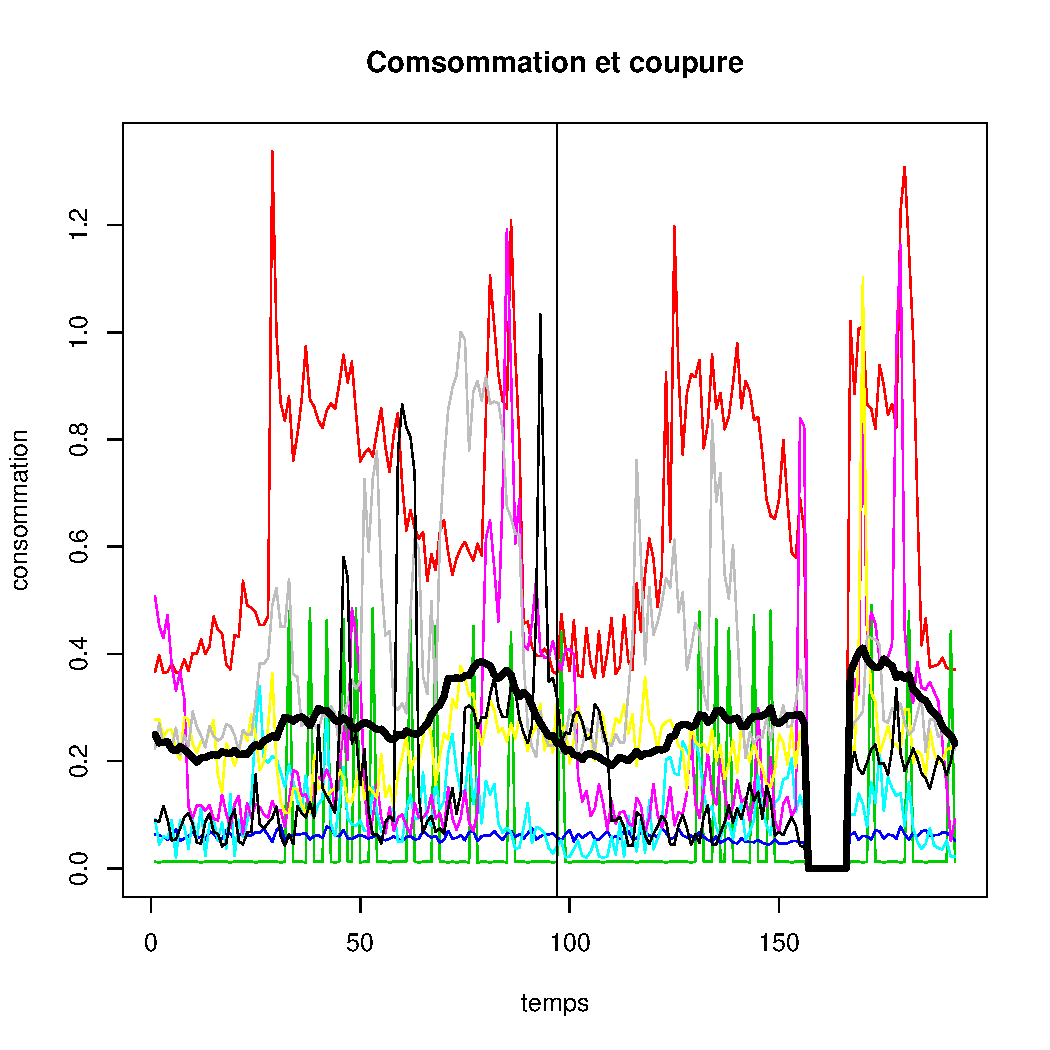
\includegraphics[width=3.5in,height=2in]{DR_gp}
\caption{{\scriptsize The different dotted and dashed lines exhibiting
    different variabilities characterize the individual 2-days DR load
    curves. Their average load curve is the bold solid line,
    representing the DR group load curve. Demand reductions are called
    between 6 and 8 pm on the days 11 and 12.}}
\label{DR_gpe2}
\end{figure}
Electric utilities hold data-mart containing $M$ non-DR customers and
their individual load curves denoted $P_j(t)$. Our aim is to
construct a control group chosen in $\{P_j(t)\}_{j=1}^M$ to
estimate the baseline on event days (example on Fig. \ref{CG_gpe2}).
\begin{figure}[!h]
\centering
%\includegraphics[]{CG_gpe2}
\caption{{\scriptsize Representation of the 3-days individual load
    curves (dotted and dashed lines) usable as control load
    curves. The average load curve of the selected control group is
    the bold solid line.}}
\label{CG_gpe2}
\end{figure}


Let $A_1,\ldots,A_M$ be $M$ indicator variables where $w_j=1$ if the
$j$th curve is in the control group. Again, this group is chosen in
such a way that the sum of its load curves is as closed as possible to
$Y(t)$. As we choose a Bayesian framework uncertainty is modeled by
probability distribution. Thus, as we don't know if the $j$th curve is
in the control group ($w_j=1$) or not ($w_j=0$) we use a Bernoulli
probability distribution $\mathrm{Ber}(\pi)$ to model this
fact. All $\{w_j\}_{j=1}^M$ random variable are supposed to be
independent.  Moreover, the value of $\pi$ is unknown and we model
it as a Beta distribution with hyper-parameter $\alpha_\pi,\beta_\pi$
($\pi\sim\mathrm{Beta}(\alpha_\pi,\beta_\pi)$).

The baseline sum $Y(t)$ (of $N$ individual) is supposed to be a
Gaussian process close to the sum of control group curve
$\frac{N}{\sum_{j=1}^{M}{w_j}}\sum_{j=1}^m w_j P_j(t)$ and we model
this fact as $Y(t)$ is a Gaussian process with mean
\begin{equation}
  \mu(w_1,\ldots,w_M) = \frac{N}{\sum_{j=1}^{M}{w_j}}\sum_{j=1}^M w_j P_j(t)
\end{equation}
and variance $\sigma^2$. This model is true for all $t$ and we use
times $t$ when $t$ is not in the event set.

To take into account that the precision $\tau=\frac{1}{\sigma^2}$ is
unknown we model it as Gamma distribution with hyper-parameters
$\alpha$ and $\beta$ ($\tau\sim\Gamma(\alpha,\beta)$).

To figure out all the parameters and their dependencies the Directed
Acyclic Graph (DAG) is given in figure \ref{dag}.
\begin{figure}[!h]
\centering
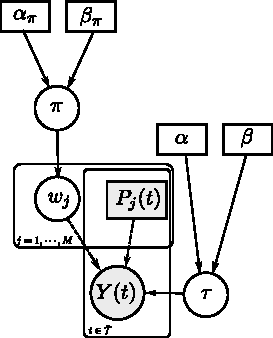
\includegraphics[]{dag}
\caption{DAG of the model: squares denote constants, circles denote
  variables. Solid arrows denote stochastic dependency, heavy dotted
  arrows denote deterministic dependency. Rounded-corner rectangles
  denote "plates" for indices. Shaded squares or circles denote
  quantities with observations}
\label{dag}
\end{figure}


Our aim is to calculate the posterior distribution of the parameter
vector $\theta^t=(w_1,\dotsc,w_M,\pi,\tau)$ (denoted as
$p(\theta|Y$). Using this posterior distribution we could make random
draw of $Y(t)$ under the posterior predictive distribution $\int
p(Y(t) | \theta) p(\theta| Y)d\theta$ in order to get credibility
interval for $Y(t)$ which are valid for all $t$, and thus on event set
$\mathcal{T}$, giving baseline estimation and credibility intervals.

We have observations of $Y(t)$ on $\bar{\mathcal{T}}$ which are
gathered in a vector $Y$.  Given the data $Y$, we can readily compute
the full conditional posterior distribution :
\begin{equation}
  \label{cond:distributionWj}
  {\mathbb P}(w_j = 1 | \theta^{(-w_j)},Y) =
  \frac{1}{1+\frac{1-\pi}{\pi}\exp\{v_j(0)-v_j(1)\}},
\end{equation}
where $\theta^{(-w_j)}$ denotes the vector of all the parameters
$\theta$ except $w_j$ and
\begin{equation*}
  v_j(z) = \exp\biggl(-\frac{\tau}{2}
  \sum_{t\in \bar{\mathcal{T}}}{
    \Bigl(Y - \frac{N}{\sum_{j=1}^{M}{w_j}}\sum_{k \not = j} w_k P_k(t) - z P_j(t)\Bigr)^2 }\biggr).
\end{equation*}
The conditional posterior distribution of the precision is
\begin{equation}
  (\tau | \theta^{(-\tau)},Y)  \sim \Gamma\biggl(\alpha+\frac{\bar T}{2},\beta + \frac{1}{2}\sum_{t\in \bar{\mathcal{T}}}{\Bigl(Y(t) - \frac{N}{\sum_{j=1}^{M}{w_j}}\sum_{k=1}^m w_k P_k(t)\Bigr)^2}\biggl).
\label{cond:distributionTau}
\end{equation}
where $\bar T$ is the number of measures of the time series in
$\bar{\mathcal{T}}$. The conditional distribution of $\pi$ is
\begin{equation}
  (\pi | \theta^{(-\pi)},Y)  \sim \mathrm{Beta}\biggl(\alpha_\pi+\sum_{j=1}^{M}{w_j} ,\beta_\pi\sum_{j=1}^{M}{(1-w_j)}\biggr).\label{cond:distributionPi}
\end{equation}

\subsection{Samples from posterior predictive distribution}
The full conditional distribution can be used to have random draw from
the posterior distribution using a Gibbs sampler: at each iteration
$k$ each component of the current parameter vector
$\theta^{(k)}=(w_1^{(k)},\dotsc,w_M^{(k)},\pi^{(k)},\tau^{(k)})^t$ is
sampled in turn from the conditional distribution (equations
\ref{cond:distributionWj}, \ref{cond:distributionTau} and
\ref{cond:distributionPi}) leading to $\theta^{(k+1)}$:
\begin{itemize}
\item sample $w_1^{(k+1)}$ from Bernoulli with parameter
  ${\mathbb P}(w_j = 1 |
  w_2^{(k)},\dotsc,w_M^{(k)},\pi^{(k)},\tau^{(k)},Y)$, see
  equation~(\ref{cond:distributionWj});
\item ...
\item sample $w_M^{(k+1)}$ from Bernoulli with parameter
  ${\mathbb P}(w_j = 1 |
  w_1^{(k+1)},\dotsc,w_{M-1}^{(k+1)},\pi^{(k)},\tau^{(k)},Y)$ see
  equation~(\ref{cond:distributionWj});
\item sample $\tau^{(k+1)}$ from $\Gamma$ with parameters
  $\alpha+\frac{\bar T}{2}$ and
  $\beta + \frac{1}{2}\sum_{t\in \bar{\mathcal{T}}}{\Bigl(Y(t) -
    \sum_{k=1}^m w^{(k+1)}_k P_k(t)\Bigr)^2}$, see
  equation~(\ref{cond:distributionTau});
\item sample $\pi^{(k+1)}$ from $\mathrm{Beta}$ with parameters
  $\alpha_\pi+\sum_{j=1}^{M}{w^{(k+1)}_j} $ and
  $\beta_\pi\sum_{j=1}^{M}{(1-w^{(k+1)}_j)}$, see
  equation~(\ref{cond:distributionPi}).
\end{itemize}
To sample from posterior predictive distribution it suffices to make
at each iteration $k$, one additional step to the previous algorithm:
sample $Y(t)^{(k+1)}$, $\forall t\in \{\mathcal{T} \cup
\bar{\mathcal{T}}\}$, from
$\mathcal{N}(\mu^{(k+1)}(t),1/\tau^{(k+1)})$ with
$\mu^{(k+1)}(t)=\sum_{j=1}^{M}{w^{(k+1)}P_j(t)}$. This sampling scheme
can be done during the Gibbs sampling or after if the whole chain
$\theta^{(1)},\dotsc,\theta^{(K)}$ is saved (note that the observed
data vector $Y$ remain the same in the posterior distribution).

From this posterior predictive sample, highest posterior density (or
credibility) intervals can be calculated as well as mean or median
curve to have a baseline estimator.
\subsection{Initialization}
To start the algorithm we need to choose the hyper-parameters
$\alpha,\beta,\alpha_p,\beta_p$. We use an empirical Bayes approach to
choose them. Recall that a $\Gamma(\alpha,\beta)$ distribution have
mean $\alpha/\beta$ and variance $\alpha/\beta^2$. Using the fact that
$Y(t)$ is a sum of $N$ load curve, we estimate it by taking the
following crude estimate $\frac{N}{M}\sum_{j=1}^{M}{P_j(t)}$ and its
variance by
$$V_t=\frac{N^2}{M^{1/2}(M-1)}\biggl(\sum_{j=1}^{M}{P_j(t)}-\frac{1}{M}\sum_{j=1}^{M}{P_j(t)}\biggr)^2.$$
The inverse of the variance estimator gives an estimator of the
precision at each time $t$. A simple (empirical) mean over
$t\in\bar{\mathcal{T}}$ of $V_t$ gives a crude estimate for the mean
of precision $\alpha/\beta$. A (empirical) variance over $T$ gives a
crude estimate of $\alpha/\beta^2$.  The variance estimator will be
certainly biased upward as all the data-mart is in the control group
but it leads to more uninformative prior which suits to our belief.

A Beta prior with parameters $\alpha_\pi$ and $\beta_\pi$ can be
interpreted as the prior observation of $\alpha_\pi-1$ successes and
$\beta_\pi-1$ failures, see for instance
\cite{bayesiandataanalysis}. As we prefer a non-informative setting we
choose $\alpha_\pi=2$ and $\beta_\pi=2$, which is equivalent to two
previous observations, one curve selected in control group and one not
selected. Recall that $M$ is usually several order of magnitude
greater than 2, thus these values of $\alpha_\pi$ and $\beta_\pi$
hyper-parameters are non-informative.

Initial value of parameters for $\tau$ can be taken from the empirical
median of $V_t$ or a random draw from $\Gamma(\alpha,\beta)$ and
$w_1,\dotsc,w_M$ can be drawn from $\mathrm{Ber}(0.5)$. These initial
values are of little importance in our simulations due to burn-in
period.

\subsection*{Monitoring convergence}
Our algorithm outputs can be easily converted in coda objects
\cite{coda} and standard analysis convergence tools can be used such
as $\hat R$ analysis (e.g. \cite{bayesiandataanalysis}), Geweke
convergence diagnostic \cite{gewekediagnostic}, Gelman shrink factor
\cite{bayesiandataanalysis} or trace of the sampled output and density
estimate of posterior distribution for $\tau$ and $\pi$. The following
and somewhat classical strategy is followed: an initial burn-in
sequence of 500 is discarded from a long sequence of iterations (for
instance 40000). On this sequence diagnostics plots are displayed:
estimated density of parameters, trace of the sampled output and
cumulative mean for $w_j^{(k)}$ over $k$. The last plot must display a
stabilization of the probability of selection if the stationary
distribution is reached. In order to monitor the convergence with the
Gelman shrink factor, we ran 15 parallel chains.  With these
diagnostics plot we can retain a starting number of iterations
$k^\star$ and applying a thinning number of 20 to ensure better
independency between successive draws of the same chain. Thanks to C++
multi-threading, running one chain or several are pretty fast,
allowing us to be very conservative in our monitoring procedure.

\section{Results}
The estimated density of $\tau$ and $\pi$ (figure
\ref{fig:densityTauPi}) are unimodal and does not show any convergence
problem.
\begin{figure}[!h]
  \centering
  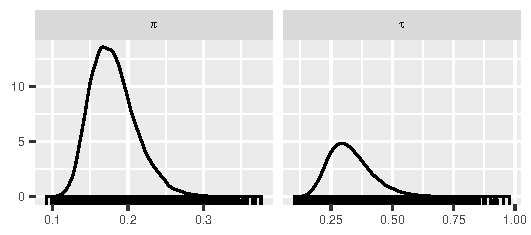
\includegraphics{density_param_tau_pi}
  \caption{Estimated posterior density for $\tau$ and $\pi$.}
  \label{fig:densityTauPi}
\end{figure}
All trajectory (figure \ref{fig:densityTauPiSumWj}) are stable and no
regime change seems to occur. The number of selected curves
($\sum_{j=1}^{M}{w_j}$) shows variations along time but no brutal
change occurs.
\begin{figure}[!h]
  \centering
  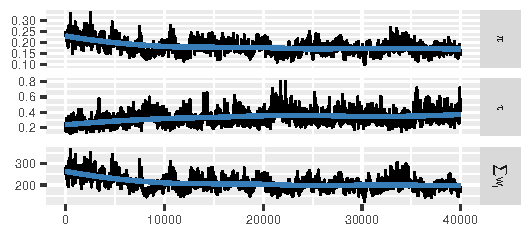
\includegraphics{trajectory_tau_pi_sum}
  \caption{Trace of output of $\tau$, $\pi$ and $\sum_j w_j$ for each iteration $k$ from 1 to $K=40000$.}
  \label{fig:densityTauPiSumWj}
\end{figure}
The convergence for estimated time in selected state for all load
curves $j\in\{1,\dotsc,M\}$ converge fast except for a few curves such
as the 1049 where the stabilization occurs at iteration
$k^\star=25000$. This choice is confirmed by the Gelman shrink factor
plot (not shown).
\begin{figure}[!h]
  \centering
  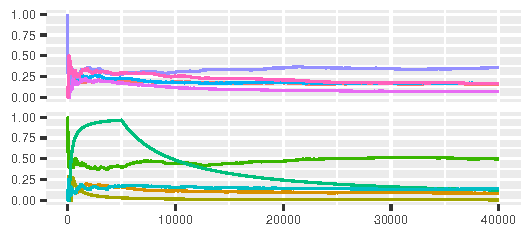
\includegraphics{meantime}
  \caption{Mean time in state ``curve $j$ in control group'' for selected $j$}
  \label{fig:meantime}
\end{figure}
Of course a more agressive starting time $k^\star$   can be selected


Using random draws from $k^\star$ up to 40000 and a thinning factor of
20 (ie using one observation every 20) we can have random draws of
posterior predictive distribution and calculate posterior mean, median
and quantile. As shown in table \ref{tab:map} posterior median is more
accurate for predicting baseline level for Mean Absolute Prediction
Error (MAPE) or Mean Square Error (MSE).
\begin{table}
 \begin{center}
  \begin{tabular}{lrrrr}\hline\hline
&\multicolumn{2}{c}{posterior mean}&\multicolumn{2}{c}{posterior median}\\\hline
          &MAPE & MSE & MAPE&  MSE\\\hline
prediction&5.04&36.28&4.92&35.25\\
all       &1.64& 7.74&1.61& 7.52\\\hline
\end{tabular}
  \end{center}
\caption{Accuracy of baseline prediction with posterior mean or median}
  \label{tab:map}
\end{table}

Our method can product high posterior density interval at a given
level, for instance the traditional level of 95\%, see figure
\ref{fig:ICY}. As expected, the confidence interval is larger for the
prediction period. The coverage is fairly good as 33 predicted
observations are within the HPD interval (on 36 to be predicted).
\begin{figure}[!h]
  \centering
  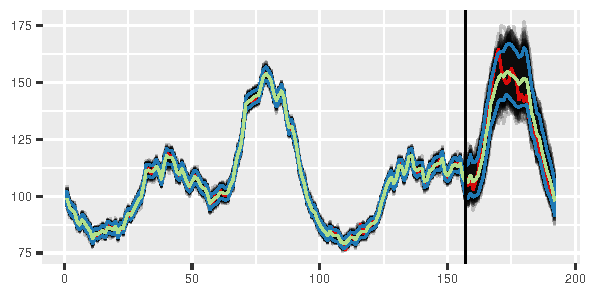
\includegraphics{ICY}
  \caption{Predicted load curves (black) using posterior predictive,
    baseline level predicted by posterior median (green) and HPD
    interval (red). The vertical line separates the fitting period and
    the prediction period.}
  \label{fig:ICY}
\end{figure}

\section{Conclusion}\label{sec:conclu}

Many DR programs have been experimented on the residential customers
to test different tariff incentives and the direct load control on
electrical appliances. The major objective is to estimate the
baseline. This is an important issue if the residential demand
reduction is introduced onto the market.

In this article, we presented baseline estimation methods relying on
new control group selection methods. While current control group
selection methods deal with the individual characteristics, our new
methods are based on the individual load curves and are easy to
implement. They significantly improve the control group selection and
give much better results than day and weather matching or regression
baseline methods. We have to keep in mind that the baselines based on
the new control group methods accurately estimate the entire day load
without using data on the hours prior to the event. This avoids
opportunities for the customers to game the process. This resultant
accuracy is major if, first, the demand reduction period varies or if
there are several demand reduction events within the day. This was
specially the case for the 2012-2013 winter in the ``Une Bretagne
d'avance'' trial where demand reductions were called between 9 and 11
am and between 6 and 8 pm. Secondly, the methods' accuracy obtained
without using the DR group data allows to quantify the anticipation or
the load report after the demand reduction event.

To select the control group, there are many advantages in considering
the individual load curves rather than the individual
characteristics. First, as the former are automatically updated, they
allow to directly include any changes related to control individuals
in the control group selection. Secondly, these new methods only
require few individual characteristics such as the localization, they
then provide a cost effective solution. Finally, bear in mind that,
the control group selection methods are not sensitive to a reasonable
variation size $N$ of the DR group.  Therefore, for all these reasons,
the control group selection methods can be used efficiently in an
operational way.

In Europe, many experiments are in progress, baseline methods could be
improved and evaluated on various customers profiles. Moreover, the
introduction of smart meters (European Electricity Directive
2009/72/EC \cite{EC_2009}) may make a large number of individual load
curves available which could be used to increase the number and the
diversity of the individual loads contributing to the control group.

Besides baseline estimation, the demand reduction forecast and the
confidence interval estimation for this quantity are major
concerns. As the demand reduction depends on the estimated baseline,
it would be also valued to have a confidence interval for the
baseline. To provide one, functional data approach could be used under
certain conditions or some astute methods suggested by \cite{interval}
could be investigated. However, this is beyond the scope of the paper
and these issues will be addressed in a future work.

\bibliographystyle{IEEEtran}
\bibliography{IEEEabrv,biblio}

%\vspace*{-7cm}
\begin{IEEEbiographynophoto}{Philippe Charpentier}
is a research engineer in statistics since 2004 within the EDF
R\&D. He is an expert in load curves analysis and particularly in
impact evaluation of rates on electrical demand. He participated in
designing several Smart Grid experiments and contributed to the
feedback.
\end{IEEEbiographynophoto}

% \vspace*{-7cm}
\begin{IEEEbiographynophoto}{Andrew Fraser}
  does independent research on inverse problems with big data as
  FraserPhysics.  He formerly chaired the Los Alamos County Board of
  Public Utilities, and he also holds a staff scientist position in
  the Computational Physics division of Los Alamos National Laboratory
  where he estimates material properties from experimental data using
  high performance computers.
\end{IEEEbiographynophoto}

% \vspace*{-7cm}
\begin{IEEEbiographynophoto}{Eric Matzner-L{\o}ber}
is Professor of statistics at Rennes University since 2007. His
research mainly focuses on merging new methodology developments with
solving real world problems in industry.
\end{IEEEbiographynophoto}

\end{document}
